\documentclass[11pt,a4paper]{article}

% ============================================================
%  PACKAGES
% ============================================================
\usepackage[utf8]{inputenc}
\usepackage[T1]{fontenc}
\usepackage{mathptmx}
\usepackage[a4paper,margin=0.6in,headheight=14pt,headsep=.15in,footskip=.3in]{geometry}
\usepackage{titlesec}
\usepackage{longtable}
\usepackage{etoolbox}
\AtBeginEnvironment{tabular}{\singlespacing}
\AtBeginEnvironment{tabularx}{\singlespacing}
\usepackage{graphicx}
\usepackage{setspace}
\usepackage{booktabs}
\usepackage{tabularx}
\usepackage{array}
\newcolumntype{L}[1]{>{\raggedright\arraybackslash}p{#1}}
\renewcommand{\tabularxcolumn}[1]{>{\raggedright\arraybackslash}p{#1}}
\usepackage{amsmath}
\usepackage{amssymb}
\usepackage{enumitem}
\usepackage{float}
\usepackage{caption}
\usepackage{tikz}
\usepackage{xcolor}
\usepackage{hyperref}
\usepackage{url}
\usepackage{cite}

\usetikzlibrary{arrows.meta,positioning}

% ============================================================
%  GENERAL STYLE
% ============================================================
\onehalfspacing
\setlength{\parindent}{0pt}
\setlength{\parskip}{6pt}
\titleformat{\section}{\fontsize{14}{18}\selectfont\bfseries}{\thesection}{.7em}{}
\titleformat{\subsection}{\fontsize{12}{16}\selectfont\bfseries}{\thesubsection}{.7em}{}
\titlespacing*{\section}{0pt}{12pt}{6pt}
\titlespacing*{\subsection}{0pt}{12pt}{6pt}
\DeclareCaptionFont{reportcaption}{\fontsize{11}{14}\selectfont}
\captionsetup{font=reportcaption,labelfont=bf,skip=6pt,hypcap=false}
\raggedbottom
\renewcommand{\topfraction}{.9}
\renewcommand{\bottomfraction}{.8}
\renewcommand{\textfraction}{.08}
\renewcommand{\floatpagefraction}{.8}
\setcounter{topnumber}{3}
\setcounter{totalnumber}{5}
\setlength{\textfloatsep}{12pt plus 2pt minus 2pt}
\setlength{\floatsep}{10pt plus 2pt minus 2pt}
\setlength{\intextsep}{10pt plus 2pt minus 2pt}
\setlist[itemize]{leftmargin=1.55em,itemsep=1pt,topsep=2pt}
\setlist[enumerate]{leftmargin=1.7em,itemsep=1pt,topsep=2pt}
\pagestyle{plain}

\hypersetup{
    hidelinks
}

\definecolor{pipelineblue}{RGB}{235,242,249}
\definecolor{pipelinegreen}{RGB}{237,247,239}

\tikzset{
  box/.style={
    rectangle, rounded corners=2pt, draw=black,
    minimum width=3.0cm, minimum height=0.68cm,
    align=center, fill=pipelineblue, font=\small
  },
  model/.style={
    rectangle, rounded corners=2pt, draw=black,
    minimum width=3.0cm, minimum height=0.68cm,
    align=center, fill=pipelinegreen, font=\small
  },
  arrow/.style={-{Latex[length=2mm]}, thick}
}

% ============================================================
%  METADATA
% ============================================================
\newcommand{\ReportTitle}{3D Target Shooter Game}
\newcommand{\CourseName}{CSE 4102: Computer Graphics and Image Processing Laboratory}

\newcommand{\FirstAuthorName}{Kazi Rifat Al Muin}
\newcommand{\FirstAuthorRoll}{2107042}

\newcommand{\SubmissionDate}{October, 2026}


\newcommand{\TeacherOne}{Md Tajmilur Rahman}
\newcommand{\TeacherOneTitle}{Lecturer}

\newcommand{\TeacherTwo}{Md. Mubtashim Abrar Nihal}
\newcommand{\TeacherTwoTitle}{Lecturer}

% ============================================================
%  DOCUMENT BEGIN
% ============================================================
\newlength{\panelheight}
\setlength{\panelheight}{2.5cm}
\newcommand{\pic}[2]{\begin{minipage}[t]{\linewidth}\centering
\ifdim\linewidth<3cm\includegraphics[width=.98\linewidth,height=1.65cm,keepaspectratio]{images/report/#1}\else\includegraphics[width=.98\linewidth,height=\panelheight,keepaspectratio]{images/report/#1}\fi
\par\vspace{1pt}{\fontsize{11}{13}\selectfont #2}\end{minipage}}
\setlength{\tabcolsep}{2pt}
\setlength{\emergencystretch}{2em}
\hypersetup{pdftitle={3D Target Shooter},pdfauthor={Kazi Rifat Al Muin, Roll 2107042}}
\begin{document}

% ----------------------------------------------------------------
%  COVER PAGE
% ----------------------------------------------------------------
\begin{titlepage}
    \setstretch{1.08}
    \pagenumbering{roman}
    \setcounter{page}{1}

    \begin{center}

        \vspace*{14pt}
        {\fontsize{12}{18}\selectfont\textbf{\CourseName}}\\
        \vspace{12pt}

        \begin{spacing}{1.4}
            {\fontsize{18}{27}\selectfont
            \textbf{\textsc{\ReportTitle}}}
        \end{spacing}


        \vspace{10pt}
        \vspace{10pt}
        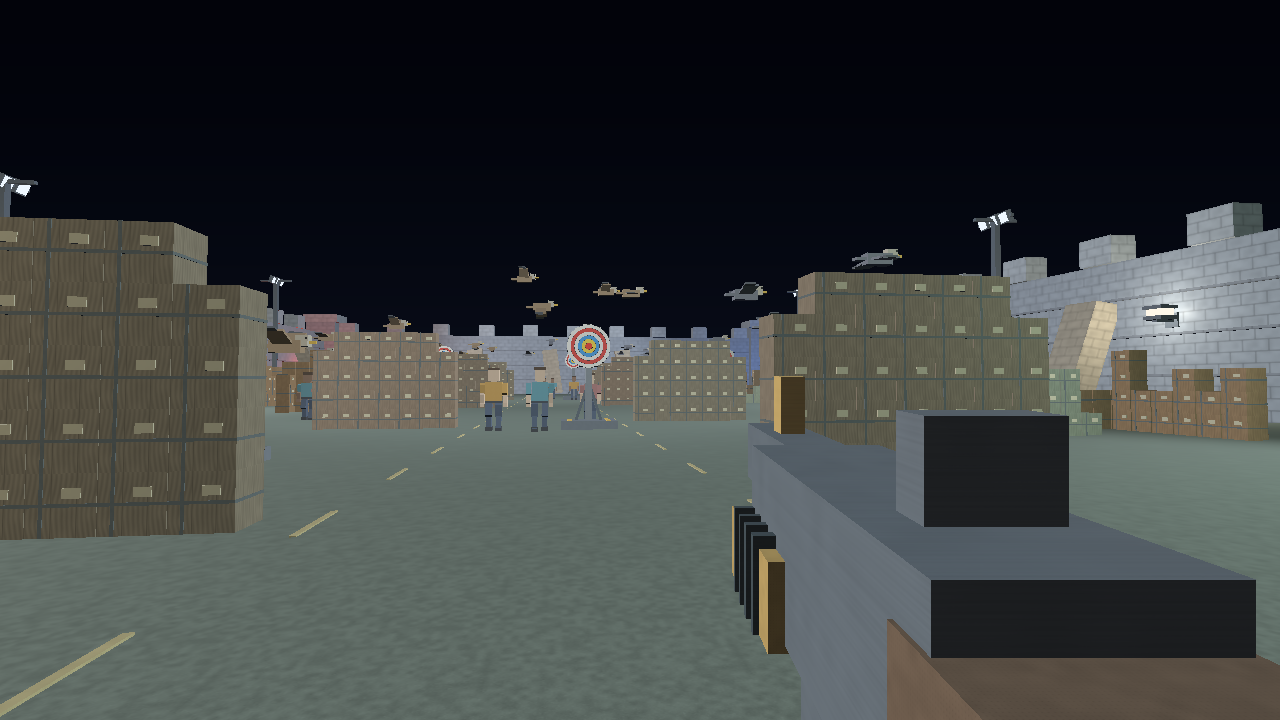
\includegraphics[width=1.65\linewidth,height=2.25in,keepaspectratio]{images/cover-level-7-night.png}\par
        \vspace{10pt}

        {\fontsize{14}{18}\selectfont By}
        \vspace{1.2\baselineskip}

        {\fontsize{14}{18}\selectfont \textbf{\FirstAuthorName}}\\
        \vspace{5pt}
        {\fontsize{12}{18}\selectfont Roll: \FirstAuthorRoll}

        \vspace{30pt}

        \IfFileExists{images/kuet_logo.png}{
            
\includegraphics[height=.9in,width=.85in,keepaspectratio]{images/kuet_logo.png}
        }{
            \fbox{\parbox[c][1.14in][c]{1.0in}{\centering KUET\\Logo}}
        }

        \vspace{20pt}

        {\fontsize{14}{16}\selectfont \textbf{Submitted To}}\\
        \vspace{20pt}

        {\fontsize{14}{15}\selectfont \textbf{\TeacherOne}}\\
        \vspace{2pt}
        {\fontsize{11}{14}\selectfont \TeacherOneTitle}\\

        \vspace{20pt}
        {\fontsize{14}{16}\selectfont \&}\par
        \vspace{6pt}
        \vspace{2pt}

        {\fontsize{14}{15}\selectfont \textbf{\TeacherTwo}}\\
        \vspace{2pt}
        {\fontsize{11}{14}\selectfont \TeacherTwoTitle}
        \vspace{30pt}

        \begin{spacing}{1.15}
            {\fontsize{12}{16}\selectfont
            \textbf{Department of Computer Science and Engineering}}\\
            {\fontsize{12}{16}\selectfont
            \textbf{Khulna University of Engineering \& Technology}}\\
            {\fontsize{12}{16}\selectfont
            \textbf{Khulna 9203, Bangladesh}}\\
            {\fontsize{12}{16}\selectfont
            \textbf{\SubmissionDate}}
        \end{spacing}

    \end{center}
\end{titlepage}
\clearpage
\pagenumbering{arabic}
\setcounter{page}{1}
\onehalfspacing
\normalsize
% Presentation report: continuous sections, 11-point body text.
\section{Introduction and Objectives}
3D Target Shooter is an interactive computer graphics project built around a three-dimensional shooting arena, moving targets and accuracy-based scoring. The seven levels progress from stationary targets to animated targets, environmental cover and non-player characters. Implemented in C++17 with OpenGL 3.3, the project demonstrates modelling with a shared cube primitive, transformations, textures, lighting, shading, animation and collision detection. These graphics concepts are integrated into a complete playable application with multiple views, weapons and gameplay modes \cite{project}.
\subsection{Relationship to the proposed project}
The proposed arena, aiming system, targets, bullets, scenery and hit effects have been implemented with multiple views and lighting conditions. Curved geometry has been simplified: cuboids are used for barrels and bullets, and 32 slices with shader-generated rings are used for target plates. Functional completion and geometric simplification are distinguished below.
\subsection{Objectives and proposal fulfilment}
The project objectives are:
\begin{enumerate}
\item Construct a complete arena and its scenery from reusable cube-based geometry.
\item Demonstrate scale, shear, rotation, translation, camera projection and normal transformation.
\item Apply textures, materials, ambient, directional, point and spot lighting, and compare flat, Gouraud and Phong shading.
\item Connect rendered geometry to animation, weapon aiming, projectile motion and ray-based collision.
\item Verify reproducible dimensions, seeded layouts, scoring, persistence and agreement between visible surfaces and gameplay interactions.
\end{enumerate}
\begin{center}\begin{tabularx}{\linewidth}{L{.20\linewidth}L{.20\linewidth}XX}\toprule
Proposed feature & Final status & Implementation & Evidence \\\midrule
Arena and scenery & Fully implemented & Floor, walls, crates, platforms & Arena/Cargo builders; Sec. 3.2--3.4\\
Gun, bullets, circular targets & Fully implemented & Cuboids and 32 target slices provide the complete playable implementation & Weapon/Target builders; Sec. 3.5--4.1\\
Motion and hit effects & Fully implemented & Sinusoids, rotation, recoil, fragments & Sec. 2.2 and 4\\
Lighting and shading & Fully implemented & Ambient, sun, points, spots; three shading modes & Shader comparisons; Sec. 7\\
Views and controls & Fully implemented & Player/arena/side/free views and mouse aiming & Camera and input logic; Sec. 5\\\bottomrule
\end{tabularx}\end{center}

World coordinates use meters; angles use degrees unless stated otherwise.
\section{Gameplay and Level Design}\subsection{Game modes, scoring and interaction}
\begin{figure}[htbp]\centering
\setlength{\panelheight}{6cm}
\begin{tabular}{p{.48\linewidth}p{.48\linewidth}}
\pic{game/release-pistol.png}{Player view: aiming and HUD.}&\pic{game/release-arena.png}{Arena view: walls, lanes and targets.}
\end{tabular}\caption{The finished game: one scene viewed from the player and arena cameras.}\end{figure}
\setlength{\panelheight}{2.5cm}
Gameplay is initiated through mode selection, after which targets are engaged from their printed front faces. A 1.5-second introduction is displayed before each Challenge level, and victory is recorded after Level 7 has been cleared. Simulation is suspended during menus, pause and results. Muzzle obstruction is evaluated independently of camera visibility, so a shot may be blocked by nearby cover even when the target is visible.
\begin{center}\begin{tabularx}{\linewidth}{lX}\toprule
Mode & Rules and persistence \\\midrule
Challenge & Seven sequential levels; accumulated score/time; eligible results after completed levels.\\
Free & Level-7 environment; 180-second session; targets return after 30 seconds; save at expiry.\\
Developer & Directly inspect any level; restart and diagnostics; no competitive record.\\
Bird's-Eye & Level-7 overview and safe click-to-observe camera; noncompetitive, no shooting.\\
Practice & Seven sandbox targets; free movement; 1.8-second target respawn; separate scoring.\\\bottomrule
\end{tabularx}\end{center}
\textbf{Hit rules:} Each target is assigned 60 health. For ring index $r=0,\ldots,5$, integer damage is calculated as $D(r)=60/(r+1)$, yielding $60,30,20,15,12,10$. A fresh target is therefore destroyed by 1--6 equal-ring hits. Rear and edge contacts are blocked without ring damage. A shared shot ID is assigned to shotgun pellets, and only the maximum ring damage from that trigger is applied. Level-mode rewards are set to $+150$ for a one-shot elimination and $+100$ otherwise; bird and human penalties are $-100$ and $-200$. In Practice, applied damage and a 100-point destruction bonus are awarded. Negative scores are retained.


Leaderboard records are separated by mode and normalized player name. Best results are saved at eligible completion boundaries; quoted names and negative scores are supported by the CSV parser.
\subsection{Seven levels and bounded target motion}
Target trajectories are specified through base position $\mathbf b$, amplitude $\mathbf a$, signed frequency $\boldsymbol\omega$, phase $\boldsymbol\phi$ and spin $s$. Shared world and gameplay builders are used throughout the seven levels. In Levels 5--7, the preceding configuration is extended so that additional difficulty is introduced without duplicating the underlying engine.
\begin{center}\begin{tabularx}{\linewidth}{crlX}\toprule
Level & Targets & Walking & New difficulty in the actual configuration \\\midrule
1 &3&Locked&Static targets at $(-5,2.4,-18),(0,2.7,-22),(5,2.4,-18)$.\\
2 &3&Locked&Center target moves horizontally: base $(0,3,-31)$, amplitude $(2.3,0,0)$.\\
3 &4&Locked&Separate X, Y and Z motion; phase-offset trajectories.\\
4 &6&Enabled&Cargo screens, longer distances, rotating targets and navigable firing positions.\\
5 &8&Enabled&Compound trajectories; eight configured birds.\\
6 &10&Enabled&Faster three-axis trajectories; sixteen configured birds.\\
7 &12&Enabled&Final pair has faster motion/spin; four birds and three humans per target (48/36).\\\bottomrule
\end{tabularx}\end{center}
\begin{equation}
 p_j(t)=b_j+a_j\sin(t\omega_j+\phi_j),\qquad \theta_y(t)=\operatorname{fmod}(ts,360).
\end{equation}
For configuration variation $v$, direction factor $d$ is assigned $-1$ for odd $v$ and $1$ otherwise. Frequency, phase and spin are then defined by
\[
 \boldsymbol\omega=(kd,1.13k,0.87kd),\quad
 \boldsymbol\phi=(0.63v,0.47v,0.81v),\quad s=s_0d.
\]
Frequencies are expressed in radians per second, while spin is expressed in degrees per second. A coordinate is held fixed when its amplitude is zero. For the Level 2 centre target, $v=0$ and $k=1.1$ give $x(1)=2.3\sin(1.1)\approx2.0498$, $y=3$ and $z=-31$. Horizontal displacement is bounded by $[-2.3,2.3]$, and the time-zero centre is $(0,3,-31)$. In subsequent levels, initial displacement is also determined by the nonzero phase terms.

\textbf{World validation:} In locked-player levels, visibility and range are checked at 32 motion samples separated by $.43$ s. In walkable levels, a $51\times91$ grid is flood-filled and reachable firing positions are required. Layout generation is retried with up to four seeds, incremented by 7919. Playability is improved by these sampled checks, although visibility is not guaranteed at every continuous instant. Target respawn is scheduled after 30 s in Free mode and 1.8 s in Practice. Configuration is defined in \path{src/levels/}; motion is evaluated by \texttt{updateTarget}.
\subsection{Level progression in the released game}
The seven Challenge levels are illustrated through the released gameplay captures. The elevated arena view is used to reveal target placement, cargo cover and the available firing lanes, while the HUD identifies the active level and recorded session state. These are gameplay snapshots rather than identical time-zero states; accumulated scores and hit feedback may therefore be visible. Increasing spatial and motion complexity is demonstrated across the sequence.
\begin{figure}[htbp]\centering
\setlength{\panelheight}{3cm}
\begin{tabular}{*{3}{p{.315\linewidth}}}
\pic{game/release-level-1.png}{Level 1: stationary targets.}&\pic{game/release-level-2.png}{Level 2: horizontal movement.}&\pic{game/release-level-3.png}{Level 3: separate motion axes.}\\
\pic{game/release-level-4.png}{Level 4: movement and cover.}&\pic{game/release-level-5.png}{Level 5: motion and bird penalties.}&\pic{game/release-level-6.png}{Level 6: increased speed and NPCs.}\\
\pic{game/release-level-7.png}{Level 7: bird and human hit feedback.}&\pic{game/release-level-7-results.png}{Final-level results.}&
\end{tabular}\caption{Progressive Challenge gameplay in Levels 1--7, followed by the final-level results screen.}\end{figure}
\section{Object Construction and 3D Transformations}\subsection{Shared geometry and model transformation}
Every world component is derived from the eight corners $(\pm0.5,\pm0.5,\pm0.5)$. The six faces are expanded into 12 triangles, giving 36 vertices with separate face normals. This mesh is stored in one VAO/VBO; transforms, colours and material parameters are supplied through each \texttt{SceneObject}. Multipart models are assembled through separate overlapping draw calls. Assembly membership is identified by the \texttt{parent} field, while the final world transform is assigned explicitly to each component.
\begin{equation}
 \mathbf p_w=M\mathbf p_l,\quad M=T R_zR_yR_xHS,\quad
 \mathbf p_c=PVM\mathbf p_l,\quad \mathbf p_{ndc}=\mathbf p_c.xyz/p_c.w.
\end{equation}
Column vectors are used, and column-major matrix storage is uploaded using \texttt{GL\_FALSE}. Thus scale is applied first and translation last. With $c=\cos\theta$, $s=\sin\theta$ and $\theta=\pi\theta_{deg}/180$:
\[
 S=\begin{bmatrix}s_x&0&0&0\\0&s_y&0&0\\0&0&s_z&0\\0&0&0&1\end{bmatrix},\quad
 H=\begin{bmatrix}1&h_{xy}&h_{xz}&0\\h_{yx}&1&h_{yz}&0\\h_{zx}&h_{zy}&1&0\\0&0&0&1\end{bmatrix},\quad
 T=\begin{bmatrix}1&0&0&t_x\\0&1&0&t_y\\0&0&1&t_z\\0&0&0&1\end{bmatrix}.
\]
\[
 R_x^{3\times3}=\begin{bmatrix}1&0&0\\0&c&-s\\0&s&c\end{bmatrix},\quad
 R_y^{3\times3}=\begin{bmatrix}c&0&s\\0&1&0\\-s&0&c\end{bmatrix},\quad
 R_z^{3\times3}=\begin{bmatrix}c&-s&0\\s&c&0\\0&0&1\end{bmatrix}.
\]
Each rotation is extended by a homogeneous fourth row and column. Points are represented with $w=1$, whereas directions and offsets are represented with $w=0$ and are unaffected by translation. At each stage, coordinates are evaluated as $p'_r=\sum_{c=0}^{3}A_{rc}p_c$. The same sequence is applied to all eight corners, allowing object bounds and rendered geometry to be derived consistently.
\textbf{Exact composition loop from \path{Transform.h}:}
\begin{verbatim}
Mat4 model = Mat4::identity();
for (const auto& stage : modelTransformStages(t))
    model = stage.matrix * model;
return model;
\end{verbatim}
\textbf{Normal transformation:} Under scale and shear, normals are transformed by $\mathbf N=\operatorname{normalize}((A^{-1})^T\mathbf n_l)$, where $A=M_{3\times3}$. For basis columns $\mathbf a,\mathbf b,\mathbf c$ and determinant $d=\mathbf a\cdot(\mathbf b\times\mathbf c)$, the normal-matrix columns are obtained as $(\mathbf b\times\mathbf c,\mathbf c\times\mathbf a,\mathbf a\times\mathbf b)/d$. Normal--surface perpendicularity is preserved, and consistent illumination is maintained on sheared parts. Shader attributes are subsequently interpolated during rasterization \cite{opengl}.
\subsection{Arena, walls and environmental construction}
A $60\times100$ m floor is used as the main arena surface. It is centred at $(0,-0.1,-50)$ and scaled by $(60,0.2,100)$, placing its upper face at $y=0$. Progression is directed along $-Z$. The environment is enclosed by four continuous 8 m walls; supports, towers and crenellations are added to establish scale and visual structure without opening the boundary.
\begin{center}\begin{tabular}{llll}\toprule
Part & Center $(x,y,z)$ & Scale $(x,y,z)$ & Yaw \\\midrule
Floor & $(0,-.1,-50)$ & $(60,.2,100)$ & $0^\circ$\\
North / South wall & $(0,4,-100)/(0,4,0)$ & $(60,8,1)$ & $0^\circ$\\
West / East wall & $(-30,4,-50)/(30,4,-50)$ & $(100,8,1)$ & $90^\circ$\\
Corner tower & $(\pm30,4.75,-100\text{ or }0)$ & $(3.5,9.5,3.5)$ & $0^\circ$\\
Corner cap & $(\pm30,10,-100\text{ or }0)$ & $(4.2,1,4.2)$ & $0^\circ$\\
End top blocks & $(x,8.75,-100\text{ or }0)$ & $(2,1.5,1.5)$ & $0^\circ$\\
Side top blocks & $(\pm30,8.75,z)$ & $(2,1.5,1.5)$ & $90^\circ$\\\bottomrule
\end{tabular}\end{center}
\begin{figure}[htbp]
\centering
\begin{tabular}{p{.237\linewidth}p{.237\linewidth}p{.237\linewidth}p{.237\linewidth}}
\pic{objects/arena-floor-slab/part-0-0.png}{Floor 1: unit.}&\pic{objects/arena-floor-slab/part-0-1.png}{Floor 2: $(60,.2,100)$.}&\pic{objects/arena-floor-slab/part-0-6.png}{Floor 3: world placement.}&\pic{objects/arena-floor-slab/complete.png}{Floor 4: final textured slab.}\\
\pic{objects/boundary-east-wall/part-0-0.png}{Wall 1: unit.}&\pic{objects/boundary-east-wall/part-0-1.png}{Wall 2: $(100,8,1)$.}&\pic{objects/boundary-east-wall/part-0-4.png}{Wall 3: $R_y(90^\circ)$.}&\pic{objects/boundary-east-wall/part-0-6.png}{Wall 4: $(30,4,-50)$.}
\end{tabular}
\caption{Arena parts are constructed from the shared cube. Scaling sets dimensions, rotation sets orientation, and translation places each component in the arena.}
\end{figure}
For the east wall, $(.5,.5,.5)\xrightarrow{S}(50,4,.5)\xrightarrow{R_y(90)}(.5,4,-50)\xrightarrow{T}(30.5,8,-100)$. Its Z span is $[-100,0]$. Thin route markers sit at $(\pm2.8,.012,z)$ with scale $(.075,.018,1.35)$. The equipment platform at $(-9,.55,-8)$ has scale $(12,1.1,3)$. Sources: \path{Arena.cpp}, \path{Environment.cpp}.
\subsection{Worked shear, rotation and ground anchoring}
Nonidentity shear and Z rotation are demonstrated by the eastern support \texttt{SUPPORT\_E\_18}. Scale $(1.5,6,2)$, shear $h_{xy}=0.22$, rotation $(0,0,-8^\circ)$ and translation $(28,2.98332977,-18)$ are assigned. The Y translation is calculated from the transformed corners so that the lowest point is anchored to the floor.
\begin{figure}[htbp]
\centering
\begin{tabular}{p{.237\linewidth}p{.237\linewidth}p{.237\linewidth}p{.237\linewidth}}
\pic{objects/boundary-sheared-stone-support/part-0-1.png}{1. Scale.}&\pic{objects/boundary-sheared-stone-support/part-0-2.png}{2. XY shear.}&\pic{objects/boundary-sheared-stone-support/part-0-5.png}{3. Z rotation.}&\pic{objects/boundary-sheared-stone-support/part-0-6.png}{4. Translation.}\end{tabular}
\caption{Support: nonidentity stages in order; X/Y rotations are identities.}
\end{figure}
\begin{center}\begin{tabular}{lll}\toprule
Operation & Calculation for local corner $(.5,.5,.5)$ & Result \\\midrule
Scale & $(1.5(.5),6(.5),2(.5))$ & $(.75,3,1)$\\
Shear & $x\leftarrow .75+.22(3)$ & $(1.41,3,1)$\\
X and Y rotations & Both angles are zero & $(1.41,3,1)$\\
Z rotation & $x=c(1.41)-s(3),\ y=s(1.41)+c(3)$ & $(1.8137973,2.7745701,1)$\\
Translation & Add $(28,2.9833298,-18)$ & $(29.8137973,5.7578999,-17)$\\\bottomrule
\end{tabular}\end{center}
Here $c=\cos(-8^\circ)=0.9902681$ and $s=-0.1391731$. The resulting matrix, rounded to seven decimals, is
\[
 M=\begin{bmatrix}
1.4854021&2.1421925&0&28\\
-.2087597&5.7578998&0&2.9833298\\
0&0&2&-18\\0&0&0&1
\end{bmatrix}.
\]
The vertical extent is obtained as $e_y=\tfrac12(|M_{10}|+|M_{11}|+|M_{12}|)\approx2.9833298$. With $t_y=e_y$, the lower bound becomes $y_{min}=t_y-e_y=0$. In the implementation, all eight corners are evaluated before translation. Both methods describe the same affine box, and its complete model matrix, including shear, is reused for collision.

\subsection{Cargo crates: deterministic multipart assembly}
A reference human height of $2.1$ m is used to establish crate side length $s=2.1/3=0.7$ m. Each crate is assembled from a wood body, two metal bands and a paper inventory plate. For the first Practice crate generated with seed 2107042, zero yaw and body centre $\mathbf b=(-21.23,.35,-20)$ are assigned.
\begin{figure}[htbp]
\centering\begin{tabular}{*{4}{p{.237\linewidth}}}
\pic{objects/cargo-crate/assembly-1.png}{1} & \pic{objects/cargo-crate/assembly-2.png}{2} & \pic{objects/cargo-crate/assembly-3.png}{3} & \pic{objects/cargo-crate/assembly-4.png}{4}\\[3pt]
\end{tabular}

\caption{Cargo assembly in builder order: (1) body, (2) vertical band, (3) horizontal band, (4) inventory plate.}
\end{figure}
\begin{center}\normalsize\begin{tabular}{rllll}\toprule
Step & Component & World center (m) & Scale (m) & Rotation (deg) \\\midrule
1 & Crate & (-21.23,0.35,-20) & (0.7,0.7,0.7) & (0,0,0) \\
2 & Crate band & (-21.426,0.35,-20) & (0.0385,0.708,0.708) & (0,0,0) \\
3 & Crate band & (-21.23,0.35,-20) & (0.708,0.0385,0.708) & (0,0,0) \\
4 & Crate inventory plate & (-21.125,0.483,-19.644) & (0.189,0.112,0.012) & (0,0,0) \\
\bottomrule\end{tabular}\end{center}

Each detail is positioned using $\mathbf p=\mathbf b+R_y(\theta)\mathbf o$ and assigned yaw $\theta$. The local offset and size relationships are specified below.
\begin{center}\begin{tabular}{lll}\toprule
Part & Local offset $\mathbf o$ & Size \\\midrule
Vertical band & $(-.28s,0,0)=(-.196,0,0)$ & $(.055s,s+.008,s+.008)$\\
Horizontal band & $(0,0,0)$ & $(s+.008,.055s,s+.008)$\\
Plate & $(.15s,.19s,.5s+.006)$ & $(.27s,.16s,.012)$\\\bottomrule
\end{tabular}\end{center}
The plate centre is obtained as $(-21.125,.483,-19.644)$ with size $(.189,.112,.012)$. Surface separation is provided by the $0.008$ and $0.006$ offsets, preventing the visible details from being placed exactly coplanar with the body. Ground contact is established by the lower bound $.35-.7/2=0$.
\textbf{Repeatable layout:} Cargo lanes are generated with \texttt{std::mt19937(seed)} at $x=-20,-15,15,20$, with jitter $(r\bmod7-3).08$. Crate spacing is set to $.735$, row depth to $z=-20-10\,row$, run length to $3+r\bmod5$, and yaw to $90(r\bmod4)$. Stack height is determined by $1+r_1\bmod3+r_2\bmod3$. Reserved corridors and target clearance are enforced to preserve movement and firing opportunities. Source: \path{Cargo.cpp}.
\subsection{Pistol assembly, aiming and recoil}
The pistol is constructed from 11 permanent cuboids. Body offset $(.32,-.25,-.68)$ and scale $(.22,.22,.56)$ produce display centre $(-12.68,1.40,-8.68)$; the grip is scaled by $(.18,.37,.20)$. For the equipment display, anchor $\mathbf c=(-13,1.65,-8)$, yaw $-90^\circ$, pitch $0^\circ$ and zero recoil are used, giving identity orientation. One component is added at each assembly stage.
\begin{figure}[htbp]
\centering\begin{tabular}{*{6}{p{.155\linewidth}}}
\pic{objects/weapon-pistol/assembly-1.png}{1} & \pic{objects/weapon-pistol/assembly-2.png}{2} & \pic{objects/weapon-pistol/assembly-3.png}{3} & \pic{objects/weapon-pistol/assembly-4.png}{4} & \pic{objects/weapon-pistol/assembly-5.png}{5} & \pic{objects/weapon-pistol/assembly-6.png}{6}\\[3pt]
\pic{objects/weapon-pistol/assembly-7.png}{7} & \pic{objects/weapon-pistol/assembly-8.png}{8} & \pic{objects/weapon-pistol/assembly-9.png}{9} & \pic{objects/weapon-pistol/assembly-10.png}{10} & \pic{objects/weapon-pistol/assembly-11.png}{11} & \\
\end{tabular}

\caption{Pistol assembly: body, grip, barrel, sight, muzzle inset, lower trigger guard, front guard, then four side details. Every added cube is retained in the following state.}
\end{figure}
\begin{center}\normalsize\begin{tabular}{rllll}\toprule
Step & Component & World center (m) & Scale (m) & Rotation (deg) \\\midrule
1 & BODY & (-12.68,1.4,-8.68) & (0.22,0.22,0.56) & (0,0,0) \\
2 & GRIP & (-12.68,1.19,-8.5) & (0.18,0.37,0.2) & (0,0,0) \\
3 & BARREL & (-12.68,1.43,-8.96) & (0.13,0.12,0.16) & (0,0,0) \\
4 & SIGHT & (-12.68,1.55,-8.89) & (0.045,0.07,0.07) & (0,0,0) \\
5 & MUZZLE\_INSET & (-12.68,1.43,-9.043) & (0.085,0.075,0.012) & (0,0,0) \\
6 & TRIGGER\_GUARD & (-12.68,1.17,-8.68) & (0.13,0.035,0.19) & (0,0,0) \\
7 & GUARD\_FRONT & (-12.68,1.25,-8.76) & (0.13,0.16,0.035) & (0,0,0) \\
8 & DETAIL\_0 & (-12.567,1.42,-8.49) & (0.015,0.13,0.013) & (0,0,0) \\
9 & DETAIL\_1 & (-12.567,1.42,-8.535) & (0.015,0.13,0.013) & (0,0,0) \\
10 & DETAIL\_2 & (-12.567,1.42,-8.58) & (0.015,0.13,0.013) & (0,0,0) \\
11 & DETAIL\_3 & (-12.567,1.42,-8.625) & (0.015,0.13,0.013) & (0,0,0) \\
\bottomrule\end{tabular}\end{center}

\textbf{Grip shear:} Before rotation, $h_{yz}=-0.3$ is applied, mapping a scaled point to $(x,y-.3z,z)$. The corner $(.5,.5,.5)$ is scaled to $(.09,.185,.10)$ and sheared to $(.09,.155,.10)$. After translation by $(-12.68,1.19,-8.5)$, the world coordinate $(-12.59,1.345,-8.4)$ is obtained. The grip slope is represented by
\[
 M_{grip}=\begin{bmatrix}.18&0&0&-12.68\\0&.37&-.06&1.19\\0&0&.20&-8.50\\0&0&0&1\end{bmatrix}.
\]
\textbf{Aiming and recoil in gameplay:} For player yaw $\psi$, pitch $\alpha$, component offset $\mathbf o$ and recoil $r$,
\[
 Q=R_y(-\psi-90)R_x(\alpha),\quad
 \mathbf p=\mathbf c+Q(\mathbf o+(0,0,.20r)),\quad
 M=T(\mathbf p)R_y(-\psi-90)R_x(\alpha)HS.
\]
The held startup pose is defined by $\mathbf c=(0,1.7,-5)$, $\psi=-90^\circ$ and $\alpha=3.8^\circ$. Body offset $(.32,-.25,-.68)$ is transformed to approximately $(.32,1.49562,-5.69507)$. A common orientation is applied to all parts, preserving the assembly during aiming. Recoil is set to $r=1$ on firing and reduced by $7\Delta t$; an emissive muzzle-flash cube is added while $r>.65$. Specular coefficient $.75$ and exponent 80 are assigned to metal parts. Cuboid barrels are used throughout. Source: \path{Weapon.cpp}.

\subsection{Shotgun and rifle assembly}
The pistol's offset-to-world relationship is also applied to the long guns. Display anchors $(-9,1.65,-8)$ and $(-5,1.65,-8)$ are used for the shotgun and rifle respectively, with yaw $-90^\circ$, zero pitch and zero recoil. A cuboid is added at each stage, and its corresponding world transform is listed in the coordinate table.
\begin{figure}[htbp]
\centering\begin{tabular}{*{8}{p{.112\linewidth}}}
\pic{objects/weapon-shotgun/assembly-1.png}{1} & \pic{objects/weapon-shotgun/assembly-2.png}{2} & \pic{objects/weapon-shotgun/assembly-3.png}{3} & \pic{objects/weapon-shotgun/assembly-4.png}{4} & \pic{objects/weapon-shotgun/assembly-5.png}{5} & \pic{objects/weapon-shotgun/assembly-6.png}{6} & \pic{objects/weapon-shotgun/assembly-7.png}{7} & \pic{objects/weapon-shotgun/assembly-8.png}{8}\\[3pt]
\pic{objects/weapon-shotgun/assembly-9.png}{9} & \pic{objects/weapon-shotgun/assembly-10.png}{10} & \pic{objects/weapon-shotgun/assembly-11.png}{11} & \pic{objects/weapon-shotgun/assembly-12.png}{12} & \pic{objects/weapon-shotgun/assembly-13.png}{13} & \pic{objects/weapon-shotgun/assembly-14.png}{14} &  & \\
\end{tabular}

\caption{Shotgun: 14 cuboids, including the wider barrel, stock, fore-end, sights, trigger guard and four fore-end bands.}
\end{figure}
\begin{center}\normalsize\begin{tabular}{rllll}\toprule
Step & Component & World center (m) & Scale (m) & Rotation (deg) \\\midrule
1 & BODY & (-8.68,1.37,-8.79) & (0.29,0.25,0.7) & (0,0,0) \\
2 & BARREL & (-8.68,1.43,-9.31) & (0.21,0.13,0.43) & (0,0,0) \\
3 & STOCK & (-8.68,1.29,-8.28) & (0.24,0.3,0.45) & (0,0,0) \\
4 & GRIP & (-8.68,1.15,-8.58) & (0.17,0.27,0.2) & (0,0,0) \\
5 & FORE\_END & (-8.68,1.3,-9.05) & (0.28,0.13,0.34) & (0,0,0) \\
6 & FRONT\_SIGHT & (-8.68,1.55,-9.34) & (0.05,0.13,0.07) & (0,0,0) \\
7 & REAR\_SIGHT & (-8.68,1.55,-8.59) & (0.13,0.1,0.06) & (0,0,0) \\
8 & MUZZLE\_INSET & (-8.68,1.43,-9.531) & (0.09,0.075,0.012) & (0,0,0) \\
9 & TRIGGER\_GUARD & (-8.68,1.17,-8.76) & (0.13,0.035,0.19) & (0,0,0) \\
10 & GUARD\_FRONT & (-8.68,1.25,-8.84) & (0.13,0.16,0.035) & (0,0,0) \\
11 & DETAIL\_0 & (-8.68,1.31,-8.95) & (0.3,0.15,0.018) & (0,0,0) \\
12 & DETAIL\_1 & (-8.68,1.31,-9.008) & (0.3,0.15,0.018) & (0,0,0) \\
13 & DETAIL\_2 & (-8.68,1.31,-9.066) & (0.3,0.15,0.018) & (0,0,0) \\
14 & DETAIL\_3 & (-8.68,1.31,-9.124) & (0.3,0.15,0.018) & (0,0,0) \\
\bottomrule\end{tabular}\end{center}

\begin{figure}[htbp]
\centering\begin{tabular}{*{8}{p{.112\linewidth}}}
\pic{objects/weapon-rifle/assembly-1.png}{1} & \pic{objects/weapon-rifle/assembly-2.png}{2} & \pic{objects/weapon-rifle/assembly-3.png}{3} & \pic{objects/weapon-rifle/assembly-4.png}{4} & \pic{objects/weapon-rifle/assembly-5.png}{5} & \pic{objects/weapon-rifle/assembly-6.png}{6} & \pic{objects/weapon-rifle/assembly-7.png}{7} & \pic{objects/weapon-rifle/assembly-8.png}{8}\\[3pt]
\pic{objects/weapon-rifle/assembly-9.png}{9} & \pic{objects/weapon-rifle/assembly-10.png}{10} & \pic{objects/weapon-rifle/assembly-11.png}{11} & \pic{objects/weapon-rifle/assembly-12.png}{12} & \pic{objects/weapon-rifle/assembly-13.png}{13} & \pic{objects/weapon-rifle/assembly-14.png}{14} & \pic{objects/weapon-rifle/assembly-15.png}{15} & \\
\end{tabular}

\caption{Rifle: 15 cuboids. The magazine is an additional sheared component; the narrower barrel and colored fore-end distinguish its silhouette.}
\end{figure}
\begin{center}\normalsize\begin{tabular}{rllll}\toprule
Step & Component & World center (m) & Scale (m) & Rotation (deg) \\\midrule
1 & BODY & (-4.68,1.37,-8.79) & (0.23,0.25,0.7) & (0,0,0) \\
2 & BARREL & (-4.68,1.43,-9.31) & (0.11,0.13,0.43) & (0,0,0) \\
3 & STOCK & (-4.68,1.29,-8.28) & (0.24,0.3,0.45) & (0,0,0) \\
4 & GRIP & (-4.68,1.15,-8.58) & (0.17,0.27,0.2) & (0,0,0) \\
5 & FORE\_END & (-4.68,1.3,-9.05) & (0.28,0.13,0.34) & (0,0,0) \\
6 & MAGAZINE & (-4.68,1.14,-8.83) & (0.15,0.35,0.24) & (0,0,0) \\
7 & FRONT\_SIGHT & (-4.68,1.55,-9.34) & (0.05,0.13,0.07) & (0,0,0) \\
8 & REAR\_SIGHT & (-4.68,1.55,-8.59) & (0.13,0.1,0.06) & (0,0,0) \\
9 & MUZZLE\_INSET & (-4.68,1.43,-9.531) & (0.09,0.075,0.012) & (0,0,0) \\
10 & TRIGGER\_GUARD & (-4.68,1.17,-8.76) & (0.13,0.035,0.19) & (0,0,0) \\
11 & GUARD\_FRONT & (-4.68,1.25,-8.84) & (0.13,0.16,0.035) & (0,0,0) \\
12 & DETAIL\_0 & (-4.68,1.31,-8.95) & (0.3,0.15,0.018) & (0,0,0) \\
13 & DETAIL\_1 & (-4.68,1.31,-9.008) & (0.3,0.15,0.018) & (0,0,0) \\
14 & DETAIL\_2 & (-4.68,1.31,-9.066) & (0.3,0.15,0.018) & (0,0,0) \\
15 & DETAIL\_3 & (-4.68,1.31,-9.124) & (0.3,0.15,0.018) & (0,0,0) \\
\bottomrule\end{tabular}\end{center}

Shear $h_{yz}=-.4$ is assigned to the long-gun grip and $h_{yz}=-.22$ to the rifle magazine. For the magazine, scale $(.15,.35,.24)$ maps $(.5,.5,.5)$ to $(.075,.175,.12)$; its Y coordinate is then modified to $.175-.22(.12)=.1486$. Translation by $(-4.68,1.14,-8.83)$ gives $(-4.605,1.2886,-8.71)$. The slanted form is therefore produced without changing the mesh. Rubber is assigned to the shotgun fore-end, while the rifle accent is given its own material assignment. Both remain attached through the common aiming transform.

\subsection{Circular targets and stands from 38 cubes}
The Practice target is centred at $(0,2.7,-19)$ with radius $r=.8$ m, thickness $.16$ m and zero yaw. Its stand is assembled from a base, pole, two braces and two warning strips. A circular plate is approximated by 32 horizontal cuboids whose widths are derived from the circle equation.
\begin{figure}[htbp]
\centering\begin{tabular}{*{8}{p{.112\linewidth}}}
\pic{objects/target/assembly-1.png}{1} & \pic{objects/target/assembly-2.png}{2} & \pic{objects/target/assembly-3.png}{3} & \pic{objects/target/assembly-4.png}{4} & \pic{objects/target/assembly-5.png}{5} & \pic{objects/target/assembly-6.png}{6} & \pic{objects/target/assembly-7.png}{7} & \pic{objects/target/assembly-8.png}{8}\\[3pt]
\pic{objects/target/assembly-9.png}{9} & \pic{objects/target/assembly-10.png}{10} & \pic{objects/target/assembly-11.png}{11} & \pic{objects/target/assembly-12.png}{12} & \pic{objects/target/assembly-13.png}{13} & \pic{objects/target/assembly-14.png}{14} & \pic{objects/target/assembly-15.png}{15} & \pic{objects/target/assembly-16.png}{16}\\[3pt]
\pic{objects/target/assembly-17.png}{17} & \pic{objects/target/assembly-18.png}{18} & \pic{objects/target/assembly-19.png}{19} & \pic{objects/target/assembly-20.png}{20} & \pic{objects/target/assembly-21.png}{21} & \pic{objects/target/assembly-22.png}{22} & \pic{objects/target/assembly-23.png}{23} & \pic{objects/target/assembly-24.png}{24}\\[3pt]
\pic{objects/target/assembly-25.png}{25} & \pic{objects/target/assembly-26.png}{26} & \pic{objects/target/assembly-27.png}{27} & \pic{objects/target/assembly-28.png}{28} & \pic{objects/target/assembly-29.png}{29} & \pic{objects/target/assembly-30.png}{30} & \pic{objects/target/assembly-31.png}{31} & \pic{objects/target/assembly-32.png}{32}\\[3pt]
\pic{objects/target/assembly-33.png}{33} & \pic{objects/target/assembly-34.png}{34} & \pic{objects/target/assembly-35.png}{35} & \pic{objects/target/assembly-36.png}{36} & \pic{objects/target/assembly-37.png}{37} & \pic{objects/target/assembly-38.png}{38} &  & \\
\end{tabular}

\caption{Target construction: 1 base, 2 pole, 3/5 braces, 4/6 strips, 7--38 plate slices. Rings are shader color.}
\end{figure}
\begin{align}
 h&=2r/32=.05, & y_i&=-r+(i+.5)h, & w_i&=2\sqrt{r^2-y_i^2},\\
 \mathbf p_i&=(0,2.7+y_i,-19), & S_i&=(w_i,.05,.16), & R_i&=R_y(\theta).
\end{align}
\begin{center}\begin{tabular}{rlll}\toprule
Slice & Local $y_i$ & Width $w_i$ & World center \\\midrule
0 & $-.775$ & $.396863$ & $(0,1.925,-19)$\\
7 & $-.425$ & $1.355544$ & $(0,2.275,-19)$\\
15 & $-.025$ & $1.599219$ & $(0,2.675,-19)$\\
16 & $.025$ & $1.599219$ & $(0,2.725,-19)$\\
31 & $.775$ & $.396863$ & $(0,3.475,-19)$\\\bottomrule
\end{tabular}\end{center}
The stand height is $H=\max(.3,2.7-.8)=1.9$. Base: center $(0,.15,-19)$, scale $(2,.3,1.5)$. Pole: $(0,.95,-19)$, scale $(.24,1.9,.24)$. For side $q=\pm1$, brace center is $(.28q,.751,-19)$, scale $(.10,1.064,.12)$, $R_z=18q$ degrees; warning-strip center is $(.7q,.307,-19)$, scale $(.16,.012,1.36)$.

\textbf{Ring continuity across slices:} Each slice has scale vector $\mathbf a=(w_i/1.6,.05/1.6,1)$ and offset vector $\mathbf b=(0,y_i/1.6,0)$. These correspond to the uniforms \texttt{patternScale} and \texttt{patternOffset}. Then $\mathbf q=\mathbf p_l\odot\mathbf a+\mathbf b$ and $\rho=2\|\mathbf q_{xy}\|$. The ring index is $\operatorname{clamp}(\lfloor6\rho\rfloor,0,5)$. Separators occur at $\operatorname{fract}(6\rho)>.95$. Only local $+Z$ faces print rings; others use $(.15,.18,.21)$. Yaw rotates the slices, normals and scoring front together. Sources: \path{Target.cpp}, \path{object.frag}.

\section{Animation, Shooting and Collision}\subsection{Projectiles and exact hit detection}
The pistol, shotgun and rifle projectiles are scaled by $(.10,.10,.25)$, $(.08,.08,.18)$ and $(.13,.13,.30)$ respectively. Colour $(1,.8,.22)$, emission $.6$ and specular coefficient $.8$ are assigned to all three. Their motion is directed from the muzzle towards the selected aim point.
\begin{figure}[htbp]
\centering
\begin{tabular}{p{.315\linewidth}p{.315\linewidth}p{.315\linewidth}}
\pic{objects/projectile-pistol/part-0-0.png}{Pistol: unit.}&\pic{objects/projectile-pistol/part-0-1.png}{Scale $(.10,.10,.25)$.}&\pic{objects/projectile-pistol/part-0-6.png}{Display center $(-12,1.17,-8.7)$.}\\
\pic{objects/projectile-shotgun/part-0-0.png}{Shotgun: unit.}&\pic{objects/projectile-shotgun/part-0-1.png}{Scale $(.08,.08,.18)$.}&\pic{objects/projectile-shotgun/part-0-6.png}{Display center $(-8,1.17,-8.7)$.}\\
\pic{objects/projectile-assault-rifle/part-0-0.png}{Rifle: unit.}&\pic{objects/projectile-assault-rifle/part-0-1.png}{Scale $(.13,.13,.30)$.}&\pic{objects/projectile-assault-rifle/part-0-6.png}{Display center $(-4,1.17,-8.7)$.}
\end{tabular}
\caption{Three projectile models: unit cube, scaled cuboid and world placement. The display direction $(0,0,-1)$ gives zero rotation.}
\end{figure}
\begin{center}\begin{tabular}{lrrrrr}\toprule
Weapon & Range (m)&Speed (m/s)&Cooldown (s)&Pellets&Spread\\\midrule
Pistol&25&42&.28&1&0\\Shotgun&18&36&.80&9&.075\\Rifle&70&65&.11&1&.009\\\bottomrule
\end{tabular}\end{center}
The muzzle is positioned at $\mathbf m=\mathbf c+Q(.32,-.22,z_m)$, with $z_m=-1.02$ for the pistol and $-1.52$ for long guns. When the nearest camera-ray contact is found at $d_a$, the aim point is set to $\mathbf a=\mathbf c+d_a\mathbf f$ and firing direction to $\mathbf d=\operatorname{normalize}(\mathbf a-\mathbf m)$. Camera--muzzle parallax is thereby accounted for. One central shotgun pellet and eight offsets $.075(\cos(2\pi i/8),\sin(2\pi i/8))$ are produced in the right/up basis. Rifle offsets are defined by $.009(\sin(2.4n),\cos(1.7n))$ for shot count $n$.

At each update, travel is calculated as $\ell=\min(v\Delta t,range-travelled)$ and shortened at the nearest collision. Position is advanced by $\mathbf p\leftarrow\mathbf p+\ell\mathbf d$. Simulation steps are limited to $1/120$ s. Visual orientation is obtained from $\theta_x=\arcsin(d_y)$ and $\theta_y=\operatorname{atan2}(-d_x,-d_z)$ in degrees, preserving alignment with the direction of travel.

\textbf{Affine-box collision:} Ray origin and direction are transformed into local coordinates as $\mathbf o_l=A^{-1}(\mathbf o-\mathbf t)$ and $\mathbf d_l=A^{-1}\mathbf d$, without renormalization. Intersections with each $[-.5,.5]$ slab are computed using $t_1=(-.5-o_l)/d_l$ and $t_2=(.5-o_l)/d_l$. A hit is accepted when accumulated entry does not exceed exit; parallel rays outside a slab are rejected. Target slices are tested after inverse yaw, and animated cuboids are tested for NPCs. Front scoring additionally requires local $d_z<0$ and contact at $z=thickness/2$. The visible target shape is therefore respected instead of its enclosing square being treated as a scoring surface.

\subsection{People, birds and transient effects}
For non-player characters, offsets are transformed by $\mathbf p=\mathbf p_{npc}+R_y(heading)R_x(fall)\mathbf o$ and component orientation by $R_y(heading)R_x(rx+fall)$. Humans are assembled from 21 cuboids and birds from 10. Rendered silhouettes and collision parts are generated by the same builders, so animated obstacles share the same geometric representation.
\begin{figure}[htbp]
\centering\begin{tabular}{*{8}{p{.112\linewidth}}}
\pic{objects/human/assembly-1.png}{1} & \pic{objects/human/assembly-2.png}{2} & \pic{objects/human/assembly-3.png}{3} & \pic{objects/human/assembly-4.png}{4} & \pic{objects/human/assembly-5.png}{5} & \pic{objects/human/assembly-6.png}{6} & \pic{objects/human/assembly-7.png}{7} & \pic{objects/human/assembly-8.png}{8}\\[3pt]
\pic{objects/human/assembly-9.png}{9} & \pic{objects/human/assembly-10.png}{10} & \pic{objects/human/assembly-11.png}{11} & \pic{objects/human/assembly-12.png}{12} & \pic{objects/human/assembly-13.png}{13} & \pic{objects/human/assembly-14.png}{14} & \pic{objects/human/assembly-15.png}{15} & \pic{objects/human/assembly-16.png}{16}\\[3pt]
\pic{objects/human/assembly-17.png}{17} & \pic{objects/human/assembly-18.png}{18} & \pic{objects/human/assembly-19.png}{19} & \pic{objects/human/assembly-20.png}{20} & \pic{objects/human/assembly-21.png}{21} &  &  & \\
\end{tabular}

\caption{Human assembly: torso, head and details, followed by the two articulated arms and legs.}
\end{figure}
\begin{figure}[htbp]
\centering\begin{tabular}{*{8}{p{.112\linewidth}}}
\pic{objects/bird/assembly-1.png}{1} & \pic{objects/bird/assembly-2.png}{2} & \pic{objects/bird/assembly-3.png}{3} & \pic{objects/bird/assembly-4.png}{4} & \pic{objects/bird/assembly-5.png}{5} & \pic{objects/bird/assembly-6.png}{6} & \pic{objects/bird/assembly-7.png}{7} & \pic{objects/bird/assembly-8.png}{8}\\[3pt]
\pic{objects/bird/assembly-9.png}{9} & \pic{objects/bird/assembly-10.png}{10} &  &  &  &  &  & \\
\end{tabular}

\caption{Bird assembly: body, head, beak, tail, wings, wing tips and eyes.}
\end{figure}
Human offsets and sizes are scaled by $q=H/1.82$ for seeded height $H\in[2.05,2.20]$. Torso offset $(0,1.12,0)$ and size $(.46,.58,.25)$ are used as reference proportions. Opposing limb swings are calculated as $22\sin(animation)$ degrees, and falling angle as $90\min(1,t/.75)^2$. Bird body size is set to $(.62,.26,.28)$. Bob $b=.045\sin(animation/2)$ and side-dependent flap $a_q=35q\sin(animation)$ are applied for $q=\pm1$. A wing centre of $(-.03,b-.35q\sin a_q,.35q\cos a_q)$ and size $(.38,.055,.64)$ produce articulated flight. Gravity 14 and pitch rate $260^\circ$/s are applied after fatal bird hits. Sources: \path{Human.cpp}, \path{Bird.cpp}.
\textbf{Effects equations:} Hit feedback is produced by $f=hitTime/.25$, with ring colour blended towards $(1,.76,.2)$ by $f/2$. On destruction, 12 fragments are emitted with $\alpha_i=2\pi i/12$, velocity $(2.4\cos\alpha_i,2+2\sin\alpha_i,1.5)$, lifetime $.75$ s and gravity 7. Blood particles are assigned gravity 13.5 and seeded sizes $.035$--$.07$, then flattened near the floor. For celebration particle $i$, age $a=t-.045(i\bmod7)$, angle $\beta=2.39996i$ and speed $u=5+1.4(i\bmod5)$ give position $(0,22,-26)+(ua\cos\beta,(5+i\bmod4)a-2.5a^2,ua\sin\beta)$. Grounding is based on the lowest transformed corner. Temporary particles are removed after expiry, and no additional score is awarded by these visual effects.

\section{Camera and User Interaction}\subsection{Views and projection}
\begin{figure}[htbp]\centering
\begin{tabular}{*{2}{p{.48\linewidth}}}
\pic{game/release-overhead.png}{Overhead: full arena and ground selection.}&\pic{game/release-observation.png}{Observation: selected ground position at eye height.}
\end{tabular}\caption{Bird's-Eye navigation connects an overview ray to a valid ground-level observation point.}\end{figure}
The same world is presented through player, elevated arena, side and free cameras. An overhead/observation pair and ground marker are provided in Bird's-Eye mode. The grounded player's position and firing restrictions are retained when inspection cameras are selected.
Given yaw $\psi$ and pitch $\alpha$, the camera forward direction is
\[
 \mathbf f=\operatorname{normalize}(\cos\psi\cos\alpha,\sin\alpha,\sin\psi\cos\alpha).
\]
Mouse input is converted to $\psi\leftarrow\psi+.12\Delta x$ and $\alpha\leftarrow\operatorname{clamp}(\alpha-.12\Delta y,-89,89)$. The camera basis is formed from $\mathbf s=\operatorname{normalize}(\mathbf f\times\mathbf u_0)$ and $\mathbf u=\mathbf s\times\mathbf f$, where $\mathbf u_0=(0,1,0)$ and $\mathbf e$ is the eye position. The view and projection matrices are expressed as
\[
 V=\begin{bmatrix}s_x&s_y&s_z&-\mathbf s\cdot\mathbf e\\u_x&u_y&u_z&-\mathbf u\cdot\mathbf e\\-f_x&-f_y&-f_z&\mathbf f\cdot\mathbf e\\0&0&0&1\end{bmatrix},\quad
 P=\begin{bmatrix}k/a&0&0&0\\0&k&0&0\\0&0&(F+n)/(n-F)&2Fn/(n-F)\\0&0&-1&0\end{bmatrix},
\]
where $k=1/\tan(FOV/2)$, aspect ratio $a=w/h$, and near/far distances are $n,F$. A $60^\circ$ perspective is used for gameplay. Isolated object views are generated with a $45^\circ$ perspective and automatic framing. Depth-dependent apparent size is preserved in both cases through perspective division.

\subsection{Interactive controls and movement}
\begin{center}\begin{tabularx}{\linewidth}{L{.17\linewidth}L{.17\linewidth}XX}\toprule
Key/button & Action & Function/logic & Visible effect \\\midrule
WASD, Shift & Walk/sprint & Ground movement and collision & Viewpoint moves at 5/9 m/s\\
Mouse & Aim & \texttt{Camera::look} & Yaw/pitch and held gun turn\\
Click/Space; 1/2/3 & Fire; weapon & \texttt{Game::fire}; session action & Projectile/recoil; gun changes\\
F1--F4; Q/E & Views; fly & \texttt{setCamera}; free movement & Player/arena/side/free view\\
F6/F7/F8 & Shading & \texttt{shadingMode=0/1/2} & Flat/Gouraud/Phong lighting\\
N; M & Night; audio & Session actions & Light rig / sound changes\\
Esc/Enter/R; Tab & Session; pointer & Session action; input loop & Pause/confirm/restart; cursor\\
Click/wheel/B & Bird's-Eye & Ground picking / zoom & Observation/overhead view\\
F5 & Snapshot & CSV request in \texttt{runScene} & Calculation file updates\\\bottomrule
\end{tabularx}\end{center}
Input is processed by \texttt{runScene} in \path{Application.cpp}. For grounded movement, the forward vector is flattened and normalized. Collision is resolved separately along X and Z in steps no larger than $.15$ m, with player bounds $x\in[-26,26]$ and $z\in[-96,-4]$. Free-camera speeds are set to 12/30 m/s and height is constrained to at least $.3$ m.

\textbf{Picking:} The overhead camera is initialized at $(0,120,-50)$ with yaw $-90^\circ$ and pitch $-89.9^\circ$. For normalized cursor $(u,v)$, the ray is calculated as $\mathbf r=\operatorname{normalize}[\mathbf f+(2u-1)a\tan30^\circ\mathbf s+(1-2v)\tan30^\circ\mathbf u]$. Ground intersection is obtained at $\mathbf e-\mathbf r(e_y/r_y)$. Unsafe or occluded positions are rejected; otherwise, the observation eye is placed 1.7 m above the selected point. Marker scale $(.9,.08,.9)$ and centre $(x,.045,z)$ are used, with a heading cube aligned to observation yaw/pitch.

\section{Texture Techniques}\subsection{Generation, mapping and sampling}
\begin{figure}[htbp]\centering
\begin{tabular}{*{3}{p{.315\linewidth}}}
\pic{game/release-masonry.png}{Masonry: repeating bricks and mortar.}&\pic{game/release-textured-environment.png}{Cargo: wood grain and bands.}&\pic{game/release-equipment.png}{Equipment: material and scale contrast.}
\end{tabular}\caption{Surface textures on the assembled arena and equipment. Geometry controls silhouette; face-local UV coordinates control surface repetition.}\end{figure}
Nine grayscale reflectance maps are generated offline by \path{tools/generate_textures.cpp}. Each map is stored as a $256\times256$ RGB P6 PPM image and loaded once into a \texttt{GL\_TEXTURE\_2D\_ARRAY} using \texttt{GL\_RGB8}. Material identity is introduced through procedural patterns while the shared cube geometry is retained. Texture generation is separated from per-frame rendering.
\begin{figure}[htbp]
\centering
\begin{tabular}{*{5}{p{.186\linewidth}}}
\pic{textures/plain.png}{Plain: 1.}&\pic{textures/concrete.png}{Concrete: 1.}&\pic{textures/masonry.png}{Masonry: .5.}&\pic{textures/gravel.png}{Gravel: .65.}&\pic{textures/wood.png}{Wood: 1.}\\
\pic{textures/metal.png}{Metal: 3.}&\pic{textures/fabric.png}{Fabric: 6.}&\pic{textures/paper.png}{Paper: 2.}&\pic{textures/rubber.png}{Rubber: 8.}&
\end{tabular}
\caption{The actual texture pixels; tiling values are repeats per scaled local meter, not image enlargement factors.}
\end{figure}
\textbf{Offline pattern formulas:} Integer hash noise starts with $n=(x\mathbin{\&}255)374761393+(y\mathbin{\&}255)668265263+seed\,2246822519$ modulo $2^{32}$, scrambles $n\leftarrow(n\oplus(n\gg13))1274126177$, then returns $((n\oplus(n\gg16))\mathbin{\&}65535)/65535$. A wrapped grid interpolates noise using $g(t)=t^2(3-2t)$ in both dimensions. Masonry staggers 128-pixel bricks on 64-pixel courses; wood uses $\sin(.49x+3\sin(2\pi y/256)+2c)$ and plank seams every 64 pixels. Concrete/gravel combine coarse/fine noise; metal varies mainly along rows; fabric alternates $(x+y)\bmod2$; rubber adds an 8-pixel grip grid. Values are clamped to $[0,1]$, multiplied by 255 and copied to RGB.

\textbf{Face-local UVs:} For local position $\mathbf p_l$, scale $\mathbf s$ and tiling $\tau$, mapping coordinates are defined by $\mathbf q=(\mathbf p_l+.5)\odot|\mathbf s|\tau$. Pairs $(q_x,q_z)$, $(q_z,q_y)$ and $(q_x,q_y)$ are assigned to Y, X and Z faces respectively. With $\tau=.65$, a 60 m floor is tiled 39 times across X and 65 times across Z. Texture placement is attached to local geometry, so rotation and translation do not cause texture swimming. Under shear, the pattern is deformed with the surface. Planar face mapping is used throughout.

\textbf{Sampling and colour:} Wrapping is set to \texttt{GL\_REPEAT}; linear magnification and trilinear mipmap minification are applied. Mip levels are generated once. Before illumination, base colour is evaluated as $\mathbf B=\mathbf C_{surface}\odot\operatorname{texture}(UV,layer)$. Plain is selected for emission $>.5$, Paper for target patterns, and the assigned material otherwise. Maps are treated as linear multipliers without automatic sRGB decoding. Nominal RGB storage is approximately 1.69 MiB for the base images and 2.25 MiB with mipmaps. Normal, roughness and displacement maps are not used.

\section{Lighting and Shading}\subsection{Ambient, directional and material lighting}
Phong reflection is evaluated in the shader from world position and the inverse-transpose normal \cite{phong}. Surface orientation is represented by normalized $\mathbf N$, viewer direction by $\mathbf V=\operatorname{normalize}(eye-position)$, and incident-light direction by $\mathbf L$ pointing towards the source. Effective RGB intensity $\mathbf C$ is obtained after attenuation and cone factors have been applied. Diffuse shape cues and view-dependent highlights are then calculated as follows.
\begin{align}
 a&=\max(\mathbf N\cdot\mathbf L,0), & \mathbf R&=2(\mathbf N\cdot\mathbf L)\mathbf N-\mathbf L,\\
 \mathbf D&=\mathbf A+\sum_j\mathbf C_j a_j,&
 \mathbf S&=\sum_{j:a_j>0}\mathbf C_j k_s\max(\mathbf R_j\cdot\mathbf V,0)^n.
\end{align}
In conventional notation, $I_a=k_aI_L$, $I_d=k_dI_L\max(\mathbf N\cdot\mathbf L,0)$ and $I_s=k_sI_L\max(\mathbf R\cdot\mathbf V,0)^n$. In the implementation, ambient/diffuse reflectance is supplied by base RGB, while $k_s,n$ are supplied by \texttt{materialSpecular} and \texttt{shininess}. Ambient colours $(.30,.32,.35)$ and $(.012,.016,.025)$ are assigned to day and night. Sun direction is normalized from $(.45,.8,.3)$ to approximately $(.466002,.828449,.310668)$. Day intensity is $(.95,.88,.73)$; night intensity is zero. Distance attenuation is not applied to the directional source.
\begin{figure}[htbp]
\centering
\begin{tabular}{p{.48\linewidth}p{.48\linewidth}}
\pic{lighting/day-2-mask-1.png}{(a) Day ambient only, mask 1.}&\pic{lighting/day-2-mask-2.png}{(b) Directional sun only, mask 2.}\\
\pic{lighting/day-2-mask-15.png}{(c) Complete day preset, mask 15.}&\pic{lighting/night-2-mask-15.png}{(d) Complete night preset, mask 15.}
\end{tabular}
\caption{Ambient fills all surfaces; the directional sun establishes orientation. Day and night use different source intensities.}
\end{figure}
For the upward floor normal $(0,1,0)$, the directional Lambert factor is $.828449$. Before texture/specular, day diffuse is approximately
\[
 (.30,.32,.35)+(.95,.88,.73)(.828449)=(1.087026,1.049035,.954768).
\]
Values may exceed one before the final clamp; there is no HDR tone-mapping operator. Default material values are $k_s=.12,n=24$; weapons $.75,80$; target plates/fixtures $.45,48$; crate-body specular $.09$ and human $.06$.
\[
 \mathbf L_{lit}=\mathbf B\odot\mathbf D+\mathbf S,\quad
 \mathbf C_{out}=\left[\operatorname{clamp}((1-e)\mathbf L_{lit}+e\mathbf B,0,1)\right]^{1/2.2}.
\]
Emission is implemented by blending towards unlit base colour with factor $e$; surrounding surfaces are illuminated only by the light sources. The daytime sun is represented by an emissive cube at $(25,35,-80)$ with scale $(4,4,4)$ and rotation $(0,25,15)^\circ$, and is omitted at night. Fixture-lens emission is set to 1 at night and 0 by day. The sky is rendered separately as $mix(horizon,zenith,smoothstep(.15,1,uv_y))$, independently of scene lighting and camera orientation.
\textbf{Shader implementation:} The diffuse accumulator and reflection direction are evaluated in \path{lighting.glsl} by the following statements. Attenuation is included in \texttt{color} before the function is called.
\begin{verbatim}
float ndotl=max(dot(N,L),0.0);
diffuse+=color*ndotl;
vec3 R=reflect(-L,N);
\end{verbatim}
When \texttt{ndotl>0.0}, \texttt{color*materialSpecular*}\allowbreak\texttt{pow(max(dot(R,V),0.0),shininess)} is added to the specular accumulator. Highlights on back-facing surfaces are excluded by this condition.

\subsection{Point lamps, stadium spots and attenuation}
Eight point lamps and six stadium spotlights are enabled in the night preset. Fixture geometry and illumination uniforms are represented separately: each stadium fixture is assembled from 12 cuboids with three lenses, but only one spotlight is assigned. Point and spot colours are set to zero during daytime. Local illumination is controlled through
\[
 \boldsymbol\delta=\mathbf p_{light}-\mathbf p,\quad d=\max(\|\boldsymbol\delta\|,.001),\quad
 \mathbf L=\boldsymbol\delta/d,\]
\[A_p=\frac1{1+.09d+.032d^2},\quad A_s=\frac1{1+.025d+.002d^2}.
\]
For a spot, $c=\operatorname{dot}(-\mathbf L,\mathbf d_{spot})$, $t=\operatorname{clamp}((c-\cos53^\circ)/(\cos32^\circ-\cos53^\circ),0,1)$ and cone intensity $I=t^2(3-2t)$. Thus the inner cone is fully lit, the penumbra is smooth and the outer region receives zero from that spotlight. Other lights may still illuminate it.
\begin{figure}[htbp]
\centering
\begin{tabular}{p{.315\linewidth}p{.315\linewidth}p{.315\linewidth}}
\pic{lighting/night-2-mask-4.png}{(a) Point family only.}&\pic{lighting/night-2-mask-8.png}{(b) Spot family only.}&\pic{lighting/night-2-mask-13.png}{(c) Ambient+points+spots.}
\end{tabular}
\caption{Night source isolation at a fixed camera; combining the families fills different regions of the same arena.}
\end{figure}
\textbf{Point example:} Directly under the warm lamp $(-18,4.7,-12)$, floor point $(-18,0,-12)$ has $d=4.7$, $\mathbf L=(0,1,0)$ and $A_p=1/(1+.423+.70688)=.469510$ approximately. Its diffuse increment is $(2.2,1.65,.9)A_p\approx(1.032922,.774692,.422559)$. This contribution joins the other light terms before texture modulation, specular reflection, emission and gamma.
\begin{figure}[htbp]\centering
\begin{tabular}{*{3}{p{.315\linewidth}}}
\pic{lighting/point-floor-offset-1.png}{Floor offset: 1 m.}&\pic{lighting/point-floor-offset-5.png}{Floor offset: 5 m.}&\pic{lighting/point-floor-offset-12.png}{Floor offset: 12 m.}
\end{tabular}\caption{Point-light falloff across the floor; both attenuation and the normal--light angle reduce the diffuse term with horizontal distance.}\end{figure}
For horizontal offset $x$ from the lamp's floor projection,
\begin{equation}
 d(x)=\sqrt{x^2+4.7^2},\qquad \mathbf N\cdot\mathbf L=\frac{4.7}{d(x)},\qquad
 \Delta\mathbf D=\frac{(2.2,1.65,.9)\,4.7}{d(x)[1+.09d(x)+.032d(x)^2]}.
\end{equation}
The spotlight's transition has zero derivative at both cone boundaries because $I'(t)=6t(1-t)$. At $c=(\cos32^\circ+\cos53^\circ)/2$, $t=.5$ and $I=.5$; this is the midpoint in cosine space, not necessarily the midpoint angle. Distance attenuation then multiplies this cone intensity.

Point positions are $(\pm18,4.7,-12)$, $(\pm28.8,5,-38)$, $(\pm28.8,5,-68)$; the rear pair is $(\pm28.8,3.2,-89)$. Colors in source order are $(2.2,1.65,.9)$, $(1.2,2,1.3)$, four $(1.7,1.6,1.4)$, then red $(2,.25,.15)$ and blue $(.25,.65,2)$ accents. Spots sit at $(\pm28,12,z)$ for $z=-16,-48,-80$, point along $\operatorname{normalize}(-x,-10,-4)$ and have color $(1.8,1.9,2.1)$.

Pole centre $(x,6,z)$ and scale $(.38,12,.38)$ are assigned to each stadium fixture. Head angles are calculated as $R_x=-\arcsin(d_y)$, $R_y=\operatorname{atan2}(d_x,d_z)$ and $R_z=0$, in degrees. Each lens is displaced by $.18\mathbf d$ from the head centre, aligning the visible fixture with its light direction.
\begin{figure}[htbp]\centering
\begin{tabular}{*{3}{p{.315\linewidth}}}
\pic{lighting/fixture-0.png}{Point fixture: warm local lamp.}&\pic{lighting/fixture-8.png}{Stadium fixture: three lenses.}&\pic{lighting/spot-angle-0.png}{Illumination along the spotlight axis.}
\end{tabular}\caption{Visible light fixtures and their illumination. Lens emission brightens the fixture itself; point/spot uniforms illuminate other surfaces.}\end{figure}

\subsection{Flat, Gouraud and Phong shading}
The same Phong \emph{reflection equation} is used in all three shading modes; the evaluation stage and interpolation method are varied \cite{phong,gouraud}. Separate cube-face normals are retained, so geometric edges remain sharp under Phong shading. Texture sampling and target-ring evaluation are performed per fragment in every mode.
\begin{figure}[htbp]
\centering
\begin{tabular}{p{.315\linewidth}p{.315\linewidth}p{.315\linewidth}}
\pic{lighting/night-0-mask-15.png}{(a) Night: flat.}&\pic{lighting/night-1-mask-15.png}{(b) Night: Gouraud.}&\pic{lighting/night-2-mask-15.png}{(c) Night: Phong.}\\
\pic{lighting/night-0-mask-15-close.png}{(d) Flat close view.}&\pic{lighting/night-1-mask-15-close.png}{(e) Gouraud close view.}&\pic{lighting/night-2-mask-15-close.png}{(f) Phong close view.}
\end{tabular}
\caption{Controlled shading comparison: each row holds scene, camera and source mask fixed. Large floor/wall triangles expose the difference under local night lights.}
\end{figure}
\begin{center}\begin{tabularx}{\linewidth}{lXX}\toprule
Mode & Evaluation and interpolation & Consequence \\\midrule
Flat (F6)&Lighting evaluated at vertices; \texttt{flat} passes the provoking vertex result unchanged over the triangle.&A local source may produce a constant triangle-sized region.\\
Gouraud (F7)&Diffuse and specular computed at vertices and interpolated across the primitive.&Smooth vertex-to-vertex variation, but a highlight between vertices can be missed.\\
Phong (F8)&Interpolate position/normal; normalize and evaluate lighting in the fragment shader.&Distance, cone and highlights respond at fragment resolution; default mode.\\\bottomrule
\end{tabularx}\end{center}
For a smooth varying $a$, perspective-correct interpolation is expressed as $a=(\sum_i\lambda_i a_i/w_i)/(\sum_i\lambda_i/w_i)$; this interpolation is bypassed for flat varyings \cite{opengl}. Smooth and flat diffuse/specular outputs are assigned in \path{object.vert}. They are selected for modes 0/1 in \path{object.frag}, while \texttt{lighting(worldPosition,worldNormal,...)} is evaluated for mode 2. Per-fragment evaluation provides finer local-light detail at the cost of additional fragment work.

\textbf{Coverage:} Two presets, three shading modes, sixteen source masks and two viewpoints form $2\times3\times16\times2=192$ lighting comparisons. Bits are ambient=1, sun=2, points=4, spots=8. Inactive families produce identical images: points/spots by day, sun by night. Sky and emissive geometry remain visible without these sources. Shadows, AO, bloom and PBR are not implemented.

\section{Implementation, Advanced Features and Verification}
Context/input are provided by GLFW and OpenGL entry points by GLAD \cite{glfw}. Input and timing are handled by \texttt{runScene}; gameplay by \texttt{Game::update/fire}; and geometry by world/level builders. The scene is submitted by \texttt{Renderer::drawArena}, with matrices uploaded by \texttt{drawTransformedCube}. Textures are managed by \texttt{TextureCache}, illumination by GLSL, and records/HUD by persistence/UI components. Each frame is processed in input, simulation, scene construction, world/sky rendering and UI order.
\subsection{Build and execution}
A 64-bit MinGW/C++17 toolchain and an OpenGL 3.3 driver are required. Compilation is performed through \texttt{build.bat}; the game is launched through \texttt{main.exe}. In the portable release directory, \texttt{TargetShooter.exe} is accompanied by \path{assets/} and \path{shaders/}.
\subsection{Advanced features and practical optimizations}
Geometry uploads are shared through one cube VBO. Uniform locations and light rigs are cached, zero-colour lights are skipped, and scene vectors are reused. Texture layers share one binding; normal matrices are computed on the CPU. One draw call is issued per cube. Procedural cargo, reachability validation, NPC penalties, ground picking, leaderboards and asynchronous calculation snapshots are provided as additional features.
\subsection{Parameter control and visual interpretation}
Motion is controlled by amplitude, frequency and spin in \path{Level*.cpp}; weapon shape by scale/shear in \path{Weapon.cpp}; and source intensity/direction in \path{Lighting.cpp}. In \path{lighting.glsl}, increased shininess narrows highlights and increased attenuation shortens light reach. Surface repetition is adjusted through texture tiling.

\subsection{Verification and reproducibility}
Transforms, collision, scoring, seeded layouts and persistence are covered by CPU tests; views, weapons and lighting are exercised by OpenGL smoke checks. Repeated same-GPU builds produced byte-identical demonstration images, and inactive source masks matched. Functional consistency is supported by these results; cross-driver rasterization differences and hardware-dependent performance remain possible.
\section{Conclusion and Demonstration}
An interactive seven-level game has been realized through geometric modelling, transformations, projection, textures, illumination and animation. Construction parameters are shared by visible geometry and collision, allowing graphics concepts to be demonstrated through gameplay and controlled comparisons. Targets remain slice approximations; weapons and projectiles remain cube assemblies. Ray intersection is used for collision and picking, while ray-traced rendering, shadows, skinning and PBR are not implemented. Curved meshes, instancing and shadows are possible extensions.

\subsection{Demonstration sequence and key concepts}
Static aiming, bounded translation and combined motion/penalties are demonstrated in Levels 1, 2 and 7 respectively. Weapon range, spread and recoil are compared through selection; spatial structure through camera switching; and night illumination through F6/F7/F8.
\textbf{Model composition:} local scale and shear are applied before world placement through $TR_zR_yR_xHS$. \textbf{Normal transformation:} perpendicularity is preserved by the inverse transpose. \textbf{Shading:} highlights between vertices may be missed by Gouraud interpolation. \textbf{Collision:} obstacles between consecutive projectile positions are detected by segment intersection. \textbf{Light isolation:} identical illumination is obtained when masks differ only in zero-intensity source families.
Project graphics and models were created by Kazi Rifat Al Muin \cite{project}; the institutional emblem is shown on the cover.



\begin{spacing}{1.2}\begin{thebibliography}{9}\raggedright
\bibitem{project} K. R. Al Muin, ``3D Target Shooter,'' GitHub, 2026. Accessed: Oct. 8, 2026. [Online]. Available: \url{https://github.com/KaziRifatAlMuin/Graphics-Target-Shooter-Game}
\bibitem{opengl} M. Segal and K. Akeley, \emph{The OpenGL Graphics System: A Specification, Version 3.3 (Core Profile)}. Khronos Group, Mar. 11, 2010. [Online]. Available: \url{https://registry.khronos.org/OpenGL/specs/gl/glspec33.core.pdf}
\bibitem{phong} B. T. Phong, ``Illumination for computer generated pictures,'' \emph{Commun. ACM}, vol. 18, no. 6, pp. 311--317, Jun. 1975, doi: \href{https://doi.org/10.1145/360825.360839}{10.1145/360825.360839}.
\bibitem{gouraud} H. Gouraud, ``Continuous shading of curved surfaces,'' \emph{IEEE Trans. Comput.}, vol. C-20, no. 6, pp. 623--629, Jun. 1971, doi: \href{https://doi.org/10.1109/T-C.1971.223313}{10.1109/T-C.1971.223313}.
\bibitem{glfw} GLFW, ``Getting started,'' \emph{GLFW 3.3 Documentation}. Accessed: Oct. 8, 2026. [Online]. Available: \url{https://www.glfw.org/docs/3.3/quick.html}
\end{thebibliography}\end{spacing}

\end{document}
